\subsection{Helios online voting system}

\subsubsection{Model}

\begin{itemize}
		\item $w$ trustees
		\item Any mumber of clients
		\item Bulleting board for communication
\end{itemize}

\subsubsection{Approach}

\begin{itemize}
		\item Admin sets up vote
		\item Trustees sahre decryption key using $n$-of-$n$ sharing (could
				also use $t$-of-$n$, but no DKG protocol implemented)
		\item Voters encrypt votes, post ballots and authenticate to BB
		\item Trustees decrypt tally
		\item ZKP to prove that votes are legitimate, and decryption is correct
\end{itemize}

\subsubsection{Audits}

\paragraph{Cast-as-intended verification}

Goal: Allow individiual to safeguard against local malicious code.

\begin{itemize}
		\item Voter encrypts ballot with some data
		\item Open ballot and verifies it using independent plattform
		\item Repeat as often as desired
		\item Then post to BB and authenticate it
\end{itemize}

\paragraph{Recorded-as-cast verification}

Goal: Allow individual to safeguard against corrupted BB.

\begin{itemize}
		\item BB allows to verify presence of ballot with encrypted vote
\end{itemize}

\paragraph{Counted-as-recorded verification}

Goal: Universal safeguard against corrupted trustees.

\begin{itemize}
		\item Check that voters are authorized on BB
		\item Check that result computed correctly (ZKP for decryption share,
				proof of correctness for decryption operation)
\end{itemize}

\section{Integrity verification}

\subsection{Model}

\begin{itemize}
		\item One writing, many reading clients
		\item Writer incrementally posts updates to service, readers query service
		\item State is large, not ideal for direct writer - reader communication
		\item Untrusted server performs operations
		\item Clients have secure backchannel $\alpha$
\end{itemize}

\subsection{Potential solutions}

\begin{itemize}
		\item Hash of object: Would need to be recomputed over full state with every update
		\item Public-key signatures: Either sign whole thing, then recomputing
				needed. Or sign updates, then all partial signatures must end
				up with client. Suscpetible to replay attacks.
		\item Merkle trees (hash trees) solve these issues
\end{itemize}

\subsection{Authenticated data structures}

\subsubsection{Model}

\begin{itemize}
		\item Generic function $F : X \times O \rightarrow X \times R$
		\item Server stores state $x \in X$
		\item Server executes operations $o \in O$
		\item Operations generate responses $r \in R$
		\item Update operations $U \subset O : \forall u \in U : F(x, u) = (x', \bot)$. Change state, no response.
		\item Query operations $Q \subset O : \forall q \in Q : F(x, q) = (x, r)$. Do not change state, have response.
\end{itemize}

\subsubsection{Interface}

\begin{itemize}
		\item $\operatorname{KeyGen}()$: Done by writer, generates public and secret key
		\item $\operatorname{Init}_F(pk, sk, x) \rightarrow (x_\sigma, \alpha)$: Writer
				transforms initial state $x$ into protected $x_\sigma$ and
				authenticator $\alpha$
		\item $\operatorname{Update}_F(pk, sk, x_\sigma, \alpha, u) \rightarrow
				(\alpha', x'_\sigma)$: Update operation changes state and
				authenticator.
		\item $\operatorname{Refresh}_F(pk, x_\sigma, \alpha, u) \rightarrow (\alpha,
				x'_\sigma)$: Server re-executes update information. May not
				produce new authenticator.
		\item $\operatorname{Query}(pk, x_\sigma, \alpha, q) \rightarrow (r,
				\phi)$: Client queries state. Produces result, and `proof' for
				result.
		\item $\operatorname{Verify}(pk, \alpha, q, r) \rightarrow True/False$:
				Client verifies if response to query is correct.
\end{itemize}

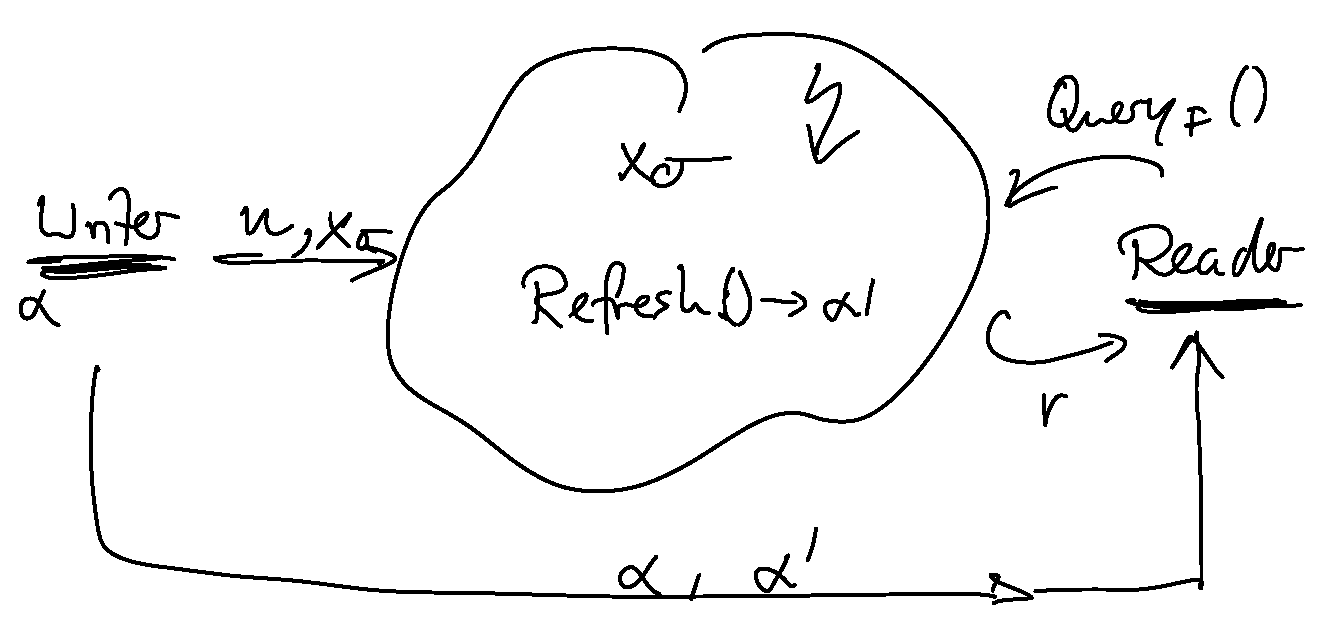
\includegraphics[width=0.8\textwidth]{12_model}
